\documentclass[conference]{IEEEtran}
\usepackage[utf8]{inputenc}
\usepackage[T1]{fontenc}
\usepackage[spanish,es-tabla,es-nodecimaldot]{babel}
\usepackage{amsmath,amssymb}
\usepackage{graphicx}
\usepackage{booktabs}
\usepackage{cite}
\usepackage{url}
\addto\captionsspanish{\renewcommand{\figurename}{Fig.}\renewcommand{\tablename}{TABLA}}
\renewcommand{\IEEEkeywordsname}{\'Indice de t\'erminos}

% Generado por tasks/generar_macros_informe.py; no editar a mano.
\newcommand{\K}{4}
\newcommand{\ahorroEns}{43.5}
\newcommand{\ahorroRegla}{38.8}
\newcommand{\anidFmacro}{+0.018}
\newcommand{\anidFmacroHi}{+0.034}
\newcommand{\anidFmacroLo}{+0.003}
\newcommand{\anidKappa}{+0.030}
\newcommand{\anidKappaHi}{+0.058}
\newcommand{\anidKappaLo}{+0.005}
\newcommand{\anidPrec}{$-$0.023}
\newcommand{\anidPrecHi}{+0.011}
\newcommand{\anidPrecLo}{$-$0.052}
\newcommand{\anidRec}{+0.047}
\newcommand{\anidRecHi}{+0.063}
\newcommand{\anidRecLo}{+0.029}
\newcommand{\aporteclima}{$-$0.020}
\newcommand{\cmaa}{8}
\newcommand{\cmab}{0}
\newcommand{\cmam}{11}
\newcommand{\cmba}{1}
\newcommand{\cmbb}{136}
\newcommand{\cmbm}{28}
\newcommand{\cmma}{13}
\newcommand{\cmmb}{20}
\newcommand{\cmmm}{123}
\newcommand{\confArbolFmacro}{0.643}
\newcommand{\confArbolKappa}{0.570}
\newcommand{\confCombFmacro}{0.666}
\newcommand{\confCombKappa}{0.593}
\newcommand{\confEnsFmacro}{0.695}
\newcommand{\confEnsKappa}{0.635}
\newcommand{\confPersFmacro}{0.646}
\newcommand{\confPersKappa}{0.545}
\newcommand{\copEns}{20.1}
\newcommand{\copInstEns}{424\,834}
\newcommand{\copInstUnInv}{19\,311}
\newcommand{\copPers}{31.2}
\newcommand{\corrirr}{0.81}
\newcommand{\corrpot}{0.89}
\newcommand{\cortebm}{9\,043}
\newcommand{\cortema}{15\,466}
\newcommand{\errinterp}{9.6}
\newcommand{\ete}{104}
\newcommand{\etr}{138}
\newcommand{\fConjA}{0.682}
\newcommand{\fConjB}{0.565}
\newcommand{\fConjC}{0.660}
\newcommand{\finalfalsosbajo}{20}
\newcommand{\finaltau}{0.80}
\newcommand{\finalvecesbajo}{156}
\newcommand{\fugaAccCon}{0.956}
\newcommand{\fugaAccSin}{0.771}
\newcommand{\fugaKappaCon}{0.922}
\newcommand{\fugaKappaSin}{0.575}
\newcommand{\gDosDias}{3}
\newcommand{\gDosErr}{25.0}
\newcommand{\gDosInv}{2.98}
\newcommand{\gDosKappa}{0.53}
\newcommand{\gUnoDias}{4}
\newcommand{\gUnoErr}{18.8}
\newcommand{\gUnoInv}{0.29}
\newcommand{\gUnoKappa}{0.67}
\newcommand{\habA}{+0.051}
\newcommand{\habB}{$-$0.125}
\newcommand{\habC}{+0.052}
\newcommand{\iecConEnsFalsosBajo}{2}
\newcommand{\iecConEnsFmacro}{0.483}
\newcommand{\iecConN}{64}
\newcommand{\iecConPersFalsosBajo}{5}
\newcommand{\iecConPersFmacro}{0.503}
\newcommand{\iecSinEnsFalsosBajo}{18}
\newcommand{\iecSinEnsFmacro}{0.692}
\newcommand{\iecSinN}{276}
\newcommand{\iecSinPersFalsosBajo}{26}
\newcommand{\iecSinPersFmacro}{0.668}
\newcommand{\iecTodosEnsFalsosBajo}{20}
\newcommand{\iecTodosEnsFmacro}{0.670}
\newcommand{\iecTodosN}{340}
\newcommand{\iecTodosPersFalsosBajo}{31}
\newcommand{\iecTodosPersFmacro}{0.657}
\newcommand{\invbajook}{0.42}
\newcommand{\invsobre}{2.6}
\newcommand{\irrte}{4.0}
\newcommand{\irrtr}{6.0}
\newcommand{\mejorconj}{C}
\newcommand{\mejorcv}{0.770}
\newcommand{\mejormodelo}{Random Forest}
\newcommand{\mejortrain}{0.888}
\newcommand{\najustes}{51}
\newcommand{\nalertasdesvio}{29}
\newcommand{\naltotest}{19}
\newcommand{\nausentes}{5}
\newcommand{\ncandidatos}{17}
\newcommand{\ncombinaciones}{9\,384}
\newcommand{\ndescarte}{8}
\newcommand{\ndiasentr}{27}
\newcommand{\ndiasprueba}{7}
\newcommand{\ndiaswf}{20}
\newcommand{\nentrena}{1275}
\newcommand{\nesperados}{3\,264}
\newcommand{\nfilas}{1615}
\newcommand{\nincompletos}{459}
\newcommand{\ninstceroscon}{64}
\newcommand{\nnoche}{1\,636}
\newcommand{\nprueba}{340}
\newcommand{\nregfaltan}{4\,110}
\newcommand{\nsobre}{42}
\newcommand{\ntodocero}{9}
\newcommand{\paltotest}{5.6}
\newcommand{\pbajotest}{48.5}
\newcommand{\pctMedio}{42.7}
\newcommand{\pctceros}{11.3}
\newcommand{\pctincompletos}{28.3}
\newcommand{\pctlEnsConf}{99.8}
\newcommand{\pctlEnsDes}{99.2}
\newcommand{\pctlMejorDes}{65}
\newcommand{\pctregfaltan}{5.7}
\newcommand{\pmediotest}{45.9}
\newcommand{\psimcoincide}{100}
\newcommand{\reglaAltoG}{0.56}
\newcommand{\reglaAltoP}{15\,696}
\newcommand{\reglaAltoPct}{30.0}
\newcommand{\reglaAltoPureza}{86.6}
\newcommand{\reglaBajoGcuatro}{0.42}
\newcommand{\reglaBajoGuno}{0.21}
\newcommand{\reglaBajoPct}{22.9}
\newcommand{\reglaBajoPureza}{99.7}
\newcommand{\silh}{0.35}
\newcommand{\simemAnioIni}{2021}
\newcommand{\simemMWFin}{2\,795}
\newcommand{\simemMWIni}{137.7}
\newcommand{\simemPartFin}{12.4}
\newcommand{\simemPartIni}{0.8}
\newcommand{\simemPlantasFin}{2\,142}
\newcommand{\simemPlantasIni}{64}
\newcommand{\spearman}{0.28}
\newcommand{\tClimAcc}{0.479}
\newcommand{\tClimFalsosBajo}{4}
\newcommand{\tClimFmacro}{0.442}
\newcommand{\tClimKappa}{0.256}
\newcommand{\tClimMWh}{10.0}
\newcommand{\tClimPrec}{0.958}
\newcommand{\tClimRec}{0.552}
\newcommand{\tCombAcc}{0.779}
\newcommand{\tCombFalsosBajo}{14}
\newcommand{\tCombFmacro}{0.670}
\newcommand{\tCombKappa}{0.603}
\newcommand{\tCombMWh}{38.4}
\newcommand{\tCombPrec}{0.901}
\newcommand{\tCombRec}{0.770}
\newcommand{\tDummyAcc}{0.056}
\newcommand{\tDummyFmacro}{0.035}
\newcommand{\tEnsAcc}{0.785}
\newcommand{\tEnsFalsosBajo}{20}
\newcommand{\tEnsFmacro}{0.670}
\newcommand{\tEnsKappa}{0.613}
\newcommand{\tEnsMWh}{57.5}
\newcommand{\tEnsPrec}{0.872}
\newcommand{\tEnsRec}{0.824}
\newcommand{\tMejorAcc}{0.782}
\newcommand{\tMejorFalsosBajo}{15}
\newcommand{\tMejorFmacro}{0.652}
\newcommand{\tMejorKappa}{0.604}
\newcommand{\tMejorMWh}{43.5}
\newcommand{\tMejorPrec}{0.894}
\newcommand{\tMejorRec}{0.770}
\newcommand{\tPersAcc}{0.756}
\newcommand{\tPersFalsosBajo}{31}
\newcommand{\tPersFmacro}{0.657}
\newcommand{\tPersKappa}{0.557}
\newcommand{\tPersMWh}{89.0}
\newcommand{\tPersPrec}{0.812}
\newcommand{\tPersRec}{0.812}
\newcommand{\umbral}{0.02}
\newcommand{\vjoblib}{1.6.0}
\newcommand{\vmatplotlib}{3.11.2}
\newcommand{\vmissingno}{0.5.2}
\newcommand{\vnumpy}{2.5.4}
\newcommand{\vpandas}{3.1.1}
\newcommand{\vpython}{3.13.3}
\newcommand{\vscikitlearn}{1.9.1}
\newcommand{\vscipy}{1.18.1}
\newcommand{\vseaborn}{0.13.2}
\newcommand{\vstatsmodels}{0.15.0}
\newcommand{\vxgboost}{3.4.1}
\newcommand{\wconv}{0.73}
\newcommand{\wfCombFmacro}{+0.029}
\newcommand{\wfCombFmacroHi}{+0.051}
\newcommand{\wfCombFmacroLo}{+0.009}
\newcommand{\wfCombKappa}{+0.042}
\newcommand{\wfCombKappaHi}{+0.078}
\newcommand{\wfCombKappaLo}{+0.008}
\newcommand{\wfCombPrec}{$-$0.018}
\newcommand{\wfCombPrecHi}{+0.024}
\newcommand{\wfCombPrecLo}{$-$0.055}
\newcommand{\wfCombRec}{+0.042}
\newcommand{\wfCombRecHi}{+0.061}
\newcommand{\wfCombRecLo}{+0.020}
\newcommand{\wfPersFmacro}{+0.049}
\newcommand{\wfPersFmacroHi}{+0.068}
\newcommand{\wfPersFmacroLo}{+0.030}
\newcommand{\wfPersKappa}{+0.089}
\newcommand{\wfPersKappaHi}{+0.116}
\newcommand{\wfPersKappaLo}{+0.065}
\newcommand{\wfPersPrec}{+0.069}
\newcommand{\wfPersPrecHi}{+0.097}
\newcommand{\wfPersPrecLo}{+0.040}
\newcommand{\wfPersRec}{+0.021}
\newcommand{\wfPersRecHi}{+0.047}
\newcommand{\wfPersRecLo}{$-$0.007}


\begin{document}

\title{Anticipar el nivel de generaci\'on de una planta fotovoltaica a 15 minutos:\\ de la persistencia a un ensamble de modelos}

\author{\IEEEauthorblockN{David Gonz\'alez Chois, Sara Castrill\'on y Juan Miguel Correa}
\IEEEauthorblockA{Anal\'itica de Datos I, Universidad Icesi, Cali, Colombia}}

\maketitle

\begin{abstract}
Una empresa de operaci\'on y mantenimiento de plantas solares necesita saber, con 15 minutos de anticipaci\'on, si la planta estar\'a en nivel bajo, medio o alto, para intervenir cuando menos energ\'ia se pierde y detectar fallas. Este trabajo construye esa base con 34 d\'ias de registros cada 15 minutos de una planta de 22 inversores: se corrigieron los inversores ausentes, se definieron los niveles por terciles del entrenamiento y se usaron solo rezagos de la potencia y del sensor. Los datos se dividieron por d\'ias en orden cronol\'ogico y se evaluaron adem\'as d\'ia a d\'ia, frente a la persistencia y la climatolog\'ia. Ning\'un modelo suelto entre \ncandidatos{} super\'o con claridad a la persistencia, as\'i que se probaron por fuerza bruta \ncombinaciones{} ensambles y se eligi\'o el m\'as consistente. El ensamble de cuatro modelos obtuvo un F1 macro de \tEnsFmacro{} y un $\kappa$ de \tEnsKappa{} (persistencia: \tPersFmacro{} y \tPersKappa{}), y redujo los falsos bajo de \tPersFalsosBajo{} a \tEnsFalsosBajo{}; corregida por sesgo de selecci\'on, su ventaja sobre la combinaci\'on persistencia-climatolog\'ia es de \anidKappa{} en $\kappa$. El clima reciente no aport\'o sobre la historia de la potencia, y el error creci\'o en los d\'ias con inversores fuera de servicio. Para la empresa, el modelo sirve para programar mantenimientos y, cuando se equivoca, como alerta de falla.
\end{abstract}

\begin{IEEEkeywords}
aprendizaje autom\'atico, energ\'ia solar fotovoltaica, ensamble de modelos, pron\'ostico de corto plazo
\end{IEEEkeywords}

\section{Introducci\'on}
Colombia lleva una d\'ecada construyendo el marco para la energ\'ia solar. La Ley 1715 de 2014 regul\'o la integraci\'on de las fuentes no convencionales al sistema energ\'etico \cite{ley1715}, y la Ley 2099 de 2021 la moderniz\'o para impulsar la transici\'on energ\'etica \cite{ley2099}. El efecto se ve en el registro de XM: la capacidad solar en operaci\'on pas\'o de \simemMWIni{}~MW en \simemAnioIni{} a \simemMWFin{}~MW en octubre de 2026, repartida en \simemPlantasFin{} plantas (eran \simemPlantasIni{}), y su participaci\'on en la capacidad en operaci\'on, de \simemPartIni{}~\% a \simemPartFin{}~\% \cite{xm}. Miles de plantas peque\~nas y medianas necesitan quien las opere y las mantenga, y ese es el nicho de una empresa de operaci\'on y mantenimiento (O\&M).

Para esa empresa, mantener bien una planta empieza por saber cu\'ando intervenirla. La potencia de una planta fotovoltaica sigue a la irradiancia, pero no solo a ella: la reducen el calentamiento del m\'odulo \cite{skoplaki}, el recorte del inversor cuando los paneles producen m\'as de lo que puede convertir \cite{good}, la suciedad \cite{diazgranados,costa} y las sombras parciales \cite{yaouba,maki}. Por eso la empresa tiene dos necesidades que dependen del mismo pron\'ostico. La primera es programar los mantenimientos en las ventanas de baja generaci\'on, para perder la menor energ\'ia posible al desconectar equipos. La segunda es detectar desv\'ios: si se esperaba un nivel alto y la planta genera bajo, algo falla. Hoy esas decisiones se toman con horarios fijos o con la regla de que lo que pasa ahora se repite, la persistencia, que a 15~min es dif\'icil de superar pero no anticipa cambios ni avisa de fallas.

La literatura ofrece herramientas para mejorar esa regla. Los modelos de aprendizaje autom\'atico, como el bosque aleatorio, han mostrado buen desempe\~no al pronosticar la potencia fotovoltaica en varios horizontes \cite{cantillo}; el pron\'ostico tambi\'en se ha planteado como un problema de clasificaci\'on por perfiles \cite{theocharides}; agrupar los d\'ias por su perfil de irradiancia ayuda a entender c\'omo se comportan los m\'odulos y el inversor en cada tipo de d\'ia \cite{santiago}; y desde hace d\'ecadas se sabe que combinar pron\'osticos mejora su exactitud \cite{clemen}. Lo que falta es llevar esas ideas a la decisi\'on concreta del t\'ecnico, que no necesita kilovatios sino un nivel, y medir con honestidad cu\'anto se gana frente a la persistencia.

Este trabajo construye esa base con datos p\'ublicos de una planta de la India \cite{kaggle}, que registra las mismas variables que cualquier sistema SCADA colombiano, y se pregunta: \textbf{P1}, ¿cu\'anto mejora el modelo a la persistencia en F1 macro, $\kappa$ y precisi\'on de bajo?; \textbf{P2}, ¿cu\'anto aporta el clima reciente por encima de la historia de la potencia?; y \textbf{P3}, ¿en qu\'e tipo de d\'ia falla m\'as el modelo y qu\'e papel tienen los inversores fuera de servicio? La Secci\'on~II describe c\'omo se prepararon los datos y se construy\'o el modelo, la III presenta los resultados, la IV responde las tres preguntas y la V propone c\'omo usarlo en la operaci\'on.

\section{Materiales y m\'etodos}
El trabajo sigui\'o las seis fases de CRISP-DM \cite{crispdm}, y esta secci\'on recorre las que convierten los registros de la planta en un pron\'ostico: los datos, su preparaci\'on, la formulaci\'on del problema, c\'omo se mide el acierto y c\'omo se eligi\'o el modelo.

\subsection{Datos}
Se us\'o la Planta~2 del conjunto p\'ublico \emph{Solar Power Generation Data} \cite{kaggle}: la potencia AC y DC de 22 inversores y un sensor de irradiancia y temperaturas (ambiente y m\'odulo), cada 15~min entre el 15 de mayo y el 17 de junio de 2020 (34 d\'ias). Sobre la malla completa de \nesperados{} instantes faltaban \nausentes{} registros completos, y en \nincompletos{} instantes con sol (\pctincompletos{}~\%) uno o m\'as inversores no report\'o, casi siempre en bloques de d\'ias seguidos. Esos huecos no son aleatorios, y por eso la preparaci\'on los trat\'o uno por uno.

\subsection{Preparaci\'on}
Lo primero fue decidir qu\'e instantes vale la pena pronosticar. Con un umbral de irradiancia de \umbral{}~kW/m$^2$ se descartaron \nnoche{} instantes de noche y crep\'usculo, que pesan alrededor del 1~\% de la potencia media con sol; la norma IEC 61724-1 \cite{iec61724} no fija este valor para pron\'ostico, as\'i que se tom\'o de los datos y se midi\'o la sensibilidad con 0.01 y 0.05~kW/m$^2$. Dentro de las horas de sol quedaban tres problemas. Los inversores ausentes se corrigieron estimando su aporte a partir de los que s\'i reportaban, porque excluirlos habr\'ia borrado un bloque entero de d\'ias; la norma admite excluir, incluir o estimar esos periodos \cite{iec61724}. Los instantes sin registro no se interpolaron: el promedio de los vecinos cambiaba la clase en el \errinterp{}~\% de los casos de prueba, justo cuando pasan nubes. Y los inversores en cero con sol se conservaron, porque tambi\'en marcan DC nula: son p\'erdidas reales que el modelo debe aprender a ver. Tras descartar \ndescarte{} filas con vac\'ios en el objetivo o en los rezagos quedaron \nfilas{} instantes.

\subsection{Formulaci\'on del problema}
Con esos datos limpios, la potencia de la planta en el instante $t$ es la suma de sus inversores,
\begin{equation}
P_t=\sum_{i=1}^{22}P^{AC}_{i,t},
\label{eq:potencia}
\end{equation}
y el nivel que la empresa necesita anticipar es el del instante siguiente,
\begin{equation}
y_{t+1}=\begin{cases}\text{bajo}, & P_{t+1}\le q_{1/3},\\ \text{medio}, & q_{1/3}<P_{t+1}\le q_{2/3},\\ \text{alto}, & P_{t+1}>q_{2/3},\end{cases}
\label{eq:clases}
\end{equation}
donde $q_{1/3}=\cortebm{}$~kW y $q_{2/3}=\cortema{}$~kW son los terciles de $P$ calculados solo con los d\'ias de entrenamiento, para que ning\'un dato de prueba defina las clases. Se clasifica por niveles y no se predicen kilovatios porque la decisi\'on del t\'ecnico es discreta: intervenir o esperar; plantear el pron\'ostico como clasificaci\'on tiene antecedentes en la literatura fotovoltaica \cite{theocharides}. Los predictores solo usan lo que se conoce en $t$,
\begin{equation}
\mathbf{x}_t=\big(h_t,\;P_{t-k},\;G_{t-k},\;T^{\mathrm{amb}}_{t-k},\;T^{\mathrm{mod}}_{t-k}\big),\quad k\in\{1,2,4\},
\label{eq:predictores}
\end{equation}
con $h_t$ la distancia a la hora de m\'axima potencia media, $G$ la irradiancia y $T$ las temperaturas. Los rezagos de 15, 30 y 60~min salen de la autocorrelaci\'on parcial de la serie, que es grande en el primer paso y peque\~na despu\'es \cite{cantillo}. La potencia DC del mismo instante se descart\'o por fuga: es casi una copia de la AC. Para responder P2 se armaron tres conjuntos: A, solo la historia de la potencia; B, solo el clima reciente; y C, ambos.

\subsection{M\'etricas}
Como la salida es una clase y no un valor en kilovatios, el MAPE, el RMSE o el $R^2$ no tienen sentido aqu\'i: miden distancias a un n\'umero continuo. Tampoco basta la exactitud, porque en la prueba la clase alto es apenas el \paltotest{}~\% de los instantes y un modelo que la ignore puede acertar mucho sin servir. Por eso se usan tres m\'etricas que responden a esos dos riesgos y al negocio:
\begin{equation}
F1_{\text{macro}}=\frac13\sum_{c}\frac{2TP_c}{2TP_c+FP_c+FN_c},
\label{eq:f1}
\end{equation}
\begin{equation}
\kappa=\frac{p_o-p_e}{1-p_e},\qquad
\text{Prec}_{\text{bajo}}=\frac{TP_{\text{bajo}}}{TP_{\text{bajo}}+FP_{\text{bajo}}},
\label{eq:kappa}
\end{equation}
donde $TP_c$, $FP_c$ y $FN_c$ son los aciertos, falsos positivos y falsos negativos de la clase $c$, $p_o$ es la exactitud y $p_e$ la exactitud esperada por azar. El F1 macro da a la clase alto el mismo peso que a las dem\'as; $\kappa$ descuenta el acierto que se obtendr\'ia por azar, que importa porque a 15~min la serie cambia poco y repetir el \'ultimo nivel ya acierta mucho; y la precisi\'on de bajo es la m\'etrica de la empresa, porque cada falso bajo la lleva a intervenir con la planta produciendo. El costo de ese error se midi\'o como la energ\'ia generada en los falsos bajo, $\sum P_{t+1}\,\Delta t$ con $\Delta t=0.25$~h, y en pesos con un precio supuesto de 350~COP/kWh.

\subsection{Validaci\'on y l\'ineas base}
Esas m\'etricas solo dicen algo si la prueba imita la operaci\'on, en la que siempre se predice el futuro con el pasado. Por eso los datos se dividieron por d\'ias en orden cronol\'ogico: \ndiasentr{} d\'ias (\nentrena{} instantes) para entrenar y los \ndiasprueba{} \'ultimos (\nprueba{}) para probar; partir por filas al azar inflaba la exactitud, porque instantes seguidos son casi copias. Los hiperpar\'ametros se eligieron dentro del entrenamiento con \texttt{TimeSeriesSplit} de 5 pliegues y F1 macro. Como siete d\'ias son pocos, se a\~nadi\'o una evaluaci\'on d\'ia a d\'ia (\emph{walk-forward}): desde el d\'ia 15 se reconstruye todo con los d\'ias anteriores y se predice solo el siguiente; los 6 primeros d\'ias sirven de desarrollo y los 14 restantes de confirmaci\'on, con intervalos de 95~\% por \emph{bootstrap} de d\'ias completos, no de filas, por la misma raz\'on. Un modelo solo se justifica si supera a lo trivial, as\'i que se midieron cuatro l\'ineas base: la clase m\'as frecuente; la persistencia, que repite el nivel de hace 15~min; la climatolog\'ia, que solo conoce la hora; y su combinaci\'on $w\,P_{t-1}+(1-w)\,\mathrm{clim}(h)$, con $w=\wconv{}$ estimado en el entrenamiento.

\subsection{Modelos y b\'usqueda del ensamble}
Frente a esas referencias compitieron \ncandidatos{} candidatos de tres familias: lineales (seis variantes de la regresi\'on log\'istica, LDA y SVM lineal calibrada), \'arboles y vecinos (\'arbol, bosque aleatorio, HistGradientBoosting, XGBoost y KNN) y modelos con agrupamiento (log\'istica con distancias a K-Means o con mezcla gaussiana, K-Means por grupos y mezcla gaussiana por clase). El modelo individual se eligi\'o con una regla fijada de antemano: aprovechar al menos el 70~\% de las ventanas bajas y, entre esos, la mayor precisi\'on de bajo en validaci\'on, con desempate por F1 macro. En la evaluaci\'on d\'ia a d\'ia se us\'o el \'arbol como referencia individual, por ser el m\'as f\'acil de leer.

Como ning\'un candidato se despeg\'o del resto, se busc\'o lo que s\'i puede aportar una combinaci\'on: modelos que se equivoquen en momentos distintos \cite{dietterich}. La b\'usqueda fue exhaustiva. Se promediaron con pesos iguales las probabilidades de todos los subconjuntos de 2 a 5 candidatos, \ncombinaciones{} en total, y cada uno se evalu\'o d\'ia a d\'ia,
\begin{equation}
\hat p_c(\mathbf{x})=\frac1M\sum_{m=1}^{M}\hat p^{(m)}_c(\mathbf{x}),\qquad \hat y=\arg\max_c \hat p_c(\mathbf{x}).
\label{eq:ensamble}
\end{equation}
Los pesos iguales siguen la evidencia de que los promedios simples rinden tanto como los ponderados \cite{clemen,wang}, y estimar pesos agrega error \cite{smith}. Con tantas combinaciones y tan pocos d\'ias, el primer puesto puede ser suerte, as\'i que no se eligi\'o el mejor de un solo ranking. Se eligi\'o la combinaci\'on que qued\'o arriba a la vez en cuatro evaluaciones (desarrollo, confirmaci\'on, primeros 10 y \'ultimos 10 d\'ias) y se midi\'o su ventaja real con selecci\'on anidada: elegir con unos d\'ias y evaluar en otros \cite{cawley}. Esta elecci\'on se aparta de la regla fijada para el individual, y por eso, siguiendo las recomendaciones de reporte para ciencia basada en aprendizaje autom\'atico \cite{reforms}, se informan la b\'usqueda completa y la ganancia corregida.

\subsection{Tipos de d\'ia y herramientas}
Para saber d\'onde falla el modelo, cada d\'ia se resumi\'o en energ\'ia, irradiaci\'on, rendimiento, hora pico, variabilidad de la irradiancia e inversores en cero, y se agrup\'o con K-Means ajustado solo con los d\'ias de entrenamiento, eligiendo $K$ con el codo y el coeficiente de silhouette \cite{santiago}. Todo se implement\'o en Python~\vpython{} \cite{python} con NumPy~\vnumpy{} \cite{numpy}, pandas~\vpandas{} \cite{pandas}, scikit-learn~\vscikitlearn{} \cite{sklearn}, XGBoost~\vxgboost{} \cite{xgboost}, SciPy~\vscipy{} \cite{scipy}, statsmodels~\vstatsmodels{} \cite{statsmodels}, Matplotlib~\vmatplotlib{} \cite{matplotlib}, seaborn~\vseaborn{} \cite{seaborn}, missingno~\vmissingno{} \cite{missingno}, joblib~\vjoblib{} \cite{joblib} e IPython \cite{ipython}, con semilla 42 en todo lo que tiene azar.

\section{Resultados}
La Tabla~\ref{tab:resultados} pone a todos los m\'etodos frente a la misma semana de prueba. La clase m\'as frecuente en entrenamiento obtuvo un F1 macro de \tDummyFmacro{}, y la climatolog\'ia, \tClimFmacro{}. La persistencia lleg\'o a \tPersFmacro{} con una precisi\'on de bajo de \tPersPrec{}, y su combinaci\'on con la climatolog\'ia, a \tCombFmacro{} y \tCombPrec{}. El mejor modelo individual, el bosque aleatorio con el conjunto C, obtuvo \tMejorFmacro{}; el ensamble, \tEnsFmacro{}, con el mayor $\kappa$ (\tEnsKappa{}) y el mayor recall de bajo (\tEnsRec{}). Con los conjuntos de variables, el F1 macro del mejor modelo fue \fConjA{} con la historia de la potencia (A), \fConjB{} con el clima reciente (B) y \fConjC{} con ambos (C).

\begin{table}[t]
\caption{Desempe\~no en la semana de prueba (\nprueba{} instantes)}
\label{tab:resultados}
\centering
\setlength{\tabcolsep}{3.2pt}
\begin{tabular}{@{}lcccccc@{}}
\toprule
M\'etodo & Exact. & F1$_{\text{m}}$ & $\kappa$ & Prec$_{\text{b}}$ & Rec$_{\text{b}}$ & FB \\
\midrule
Clase m\'as frecuente & \tDummyAcc & \tDummyFmacro & 0.000 & -- & -- & -- \\
Climatolog\'ia & \tClimAcc & \tClimFmacro & \tClimKappa & \textbf{\tClimPrec} & \tClimRec & \textbf{\tClimFalsosBajo} \\
Persistencia & \tPersAcc & \tPersFmacro & \tPersKappa & \tPersPrec & \tPersRec & \tPersFalsosBajo \\
Persist.\ + climatol. & \tCombAcc & \tCombFmacro & \tCombKappa & \tCombPrec & \tCombRec & \tCombFalsosBajo \\
Bosque aleatorio (C) & \tMejorAcc & \tMejorFmacro & \tMejorKappa & \tMejorPrec & \tMejorRec & \tMejorFalsosBajo \\
Ensamble (4 modelos) & \textbf{\tEnsAcc} & \textbf{\tEnsFmacro} & \textbf{\tEnsKappa} & \tEnsPrec & \textbf{\tEnsRec} & \tEnsFalsosBajo \\
\bottomrule
\end{tabular}

\vspace{2pt}
\parbox{\columnwidth}{\footnotesize F1$_{\text{m}}$: F1 macro; Prec$_{\text{b}}$ y Rec$_{\text{b}}$: precisi\'on y recall de bajo; FB: falsos bajo. En negrita, el mejor valor de cada columna.}
\end{table}

Todas esas cifras salen de una sola semana, y esa semana fue distinta de las que vio el modelo: su energ\'ia media fue de \ete{}~MWh por d\'ia frente a \etr{} en entrenamiento, y su irradiaci\'on, de \irrte{} frente a \irrtr{}~kWh/m$^2$ por d\'ia. En los \ndiaswf{} d\'ias de la evaluaci\'on d\'ia a d\'ia, que cubren otras condiciones, el ensamble obtuvo en confirmaci\'on un F1 macro de \confEnsFmacro{} y un $\kappa$ de \confEnsKappa{}, frente a \confPersFmacro{} y \confPersKappa{} de la persistencia, \confCombFmacro{} y \confCombKappa{} de la combinaci\'on y \confArbolFmacro{} y \confArbolKappa{} del \'arbol. Frente a la persistencia, las diferencias fueron \wfPersFmacro{} [\wfPersFmacroLo{}; \wfPersFmacroHi{}] en F1 macro, \wfPersKappa{} [\wfPersKappaLo{}; \wfPersKappaHi{}] en $\kappa$ y \wfPersPrec{} [\wfPersPrecLo{}; \wfPersPrecHi{}] en precisi\'on de bajo; frente a la combinaci\'on, \wfCombFmacro{} [\wfCombFmacroLo{}; \wfCombFmacroHi{}], \wfCombKappa{} [\wfCombKappaLo{}; \wfCombKappaHi{}] y \wfCombPrec{} [\wfCombPrecLo{}; \wfCombPrecHi{}].

Esas cifras corresponden a una combinaci\'on concreta entre \ncombinaciones{}, y la Fig.~\ref{fig:combinatoria} muestra c\'omo se reparti\'o la b\'usqueda. La correlaci\'on de Spearman entre el F1 macro en desarrollo y en confirmaci\'on fue de \spearman{}, y la combinaci\'on con mejor desarrollo qued\'o en el percentil \pctlMejorDes{} de confirmaci\'on. El ensamble elegido (bosque aleatorio, log\'istica ElasticNet, SVM lineal calibrada y log\'istica con distancias a K-Means) qued\'o en el percentil \pctlEnsDes{} en desarrollo y \pctlEnsConf{} en confirmaci\'on. Con la selecci\'on anidada, la ventaja del procedimiento sobre la combinaci\'on persistencia-climatolog\'ia fue de \anidFmacro{} [\anidFmacroLo{}; \anidFmacroHi{}] en F1 macro y \anidKappa{} [\anidKappaLo{}; \anidKappaHi{}] en $\kappa$.

\begin{figure}[t]
\centering
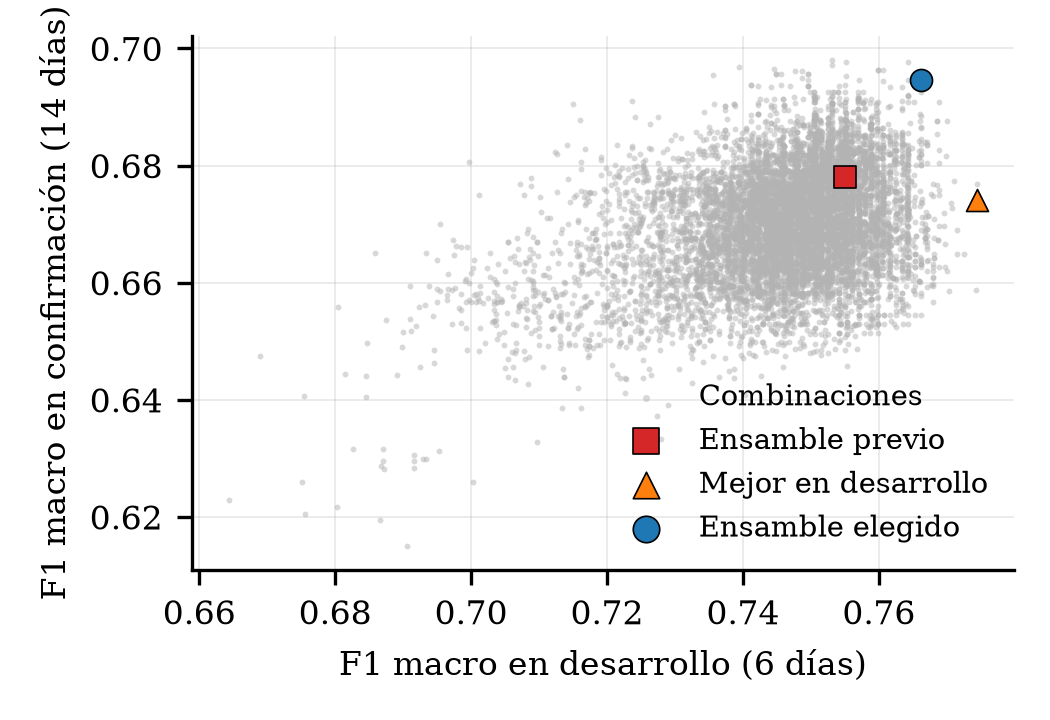
\includegraphics[width=\columnwidth]{fig_combinatoria.png}
\caption{F1 macro de las \ncombinaciones{} combinaciones de 2 a 5 modelos en los d\'ias de desarrollo y de confirmaci\'on de la evaluaci\'on d\'ia a d\'ia. El ensamble elegido queda en el extremo superior derecho; el mejor en desarrollo no.}
\label{fig:combinatoria}
\end{figure}

Dentro de la semana de prueba, la matriz de confusi\'on del ensamble (Fig.~\ref{fig:confusion}) concentra los errores entre clases vecinas: \cmbm{} instantes bajos se anunciaron como medios y \cmmb{} medios como bajos, \cmam{} de los \naltotest{} altos se anunciaron como medios y ninguno alto como bajo. El ensamble anunci\'o bajo \finalvecesbajo{} veces, con \finalfalsosbajo{} falsos bajo que suman \tEnsMWh{}~MWh (\copEns{} millones de COP si se desconecta la planta completa) frente a \tPersMWh{}~MWh (\copPers{} millones) de la persistencia. En los \nsobre{} instantes en que anunci\'o un nivel m\'as alto que el real hab\'ia en promedio \invsobre{} inversores en cero, frente a \invbajook{} en los bajos bien acertados.

\begin{figure}[t]
\centering
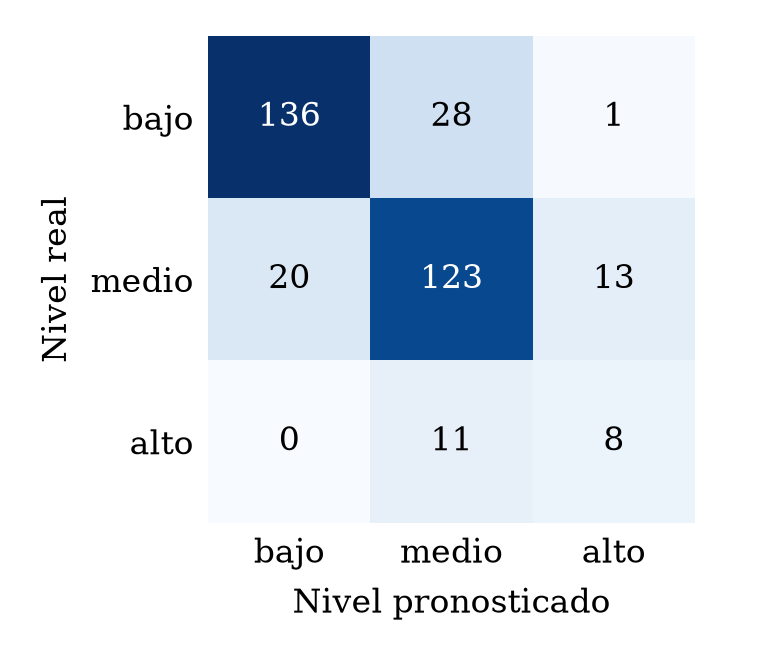
\includegraphics[width=0.72\columnwidth]{fig_confusion.png}
\caption{Matriz de confusi\'on del ensamble en la semana de prueba (\nprueba{} instantes).}
\label{fig:confusion}
\end{figure}

Por \'ultimo, K-Means separ\'o los d\'ias de entrenamiento en $K=\K{}$ grupos (silhouette de \silh{}; Fig.~\ref{fig:grupos}), de los que solo dos aparecen en la prueba. En los \gUnoDias{} d\'ias nublados con pocas p\'erdidas, el error fue de \gUnoErr{}~\% ($\kappa=\gUnoKappa{}$, \gUnoInv{} inversores en cero en promedio); en los \gDosDias{} d\'ias parcialmente nublados con p\'erdidas, de \gDosErr{}~\% ($\kappa=\gDosKappa{}$, \gDosInv{} inversores en cero).

\begin{figure}[t]
\centering
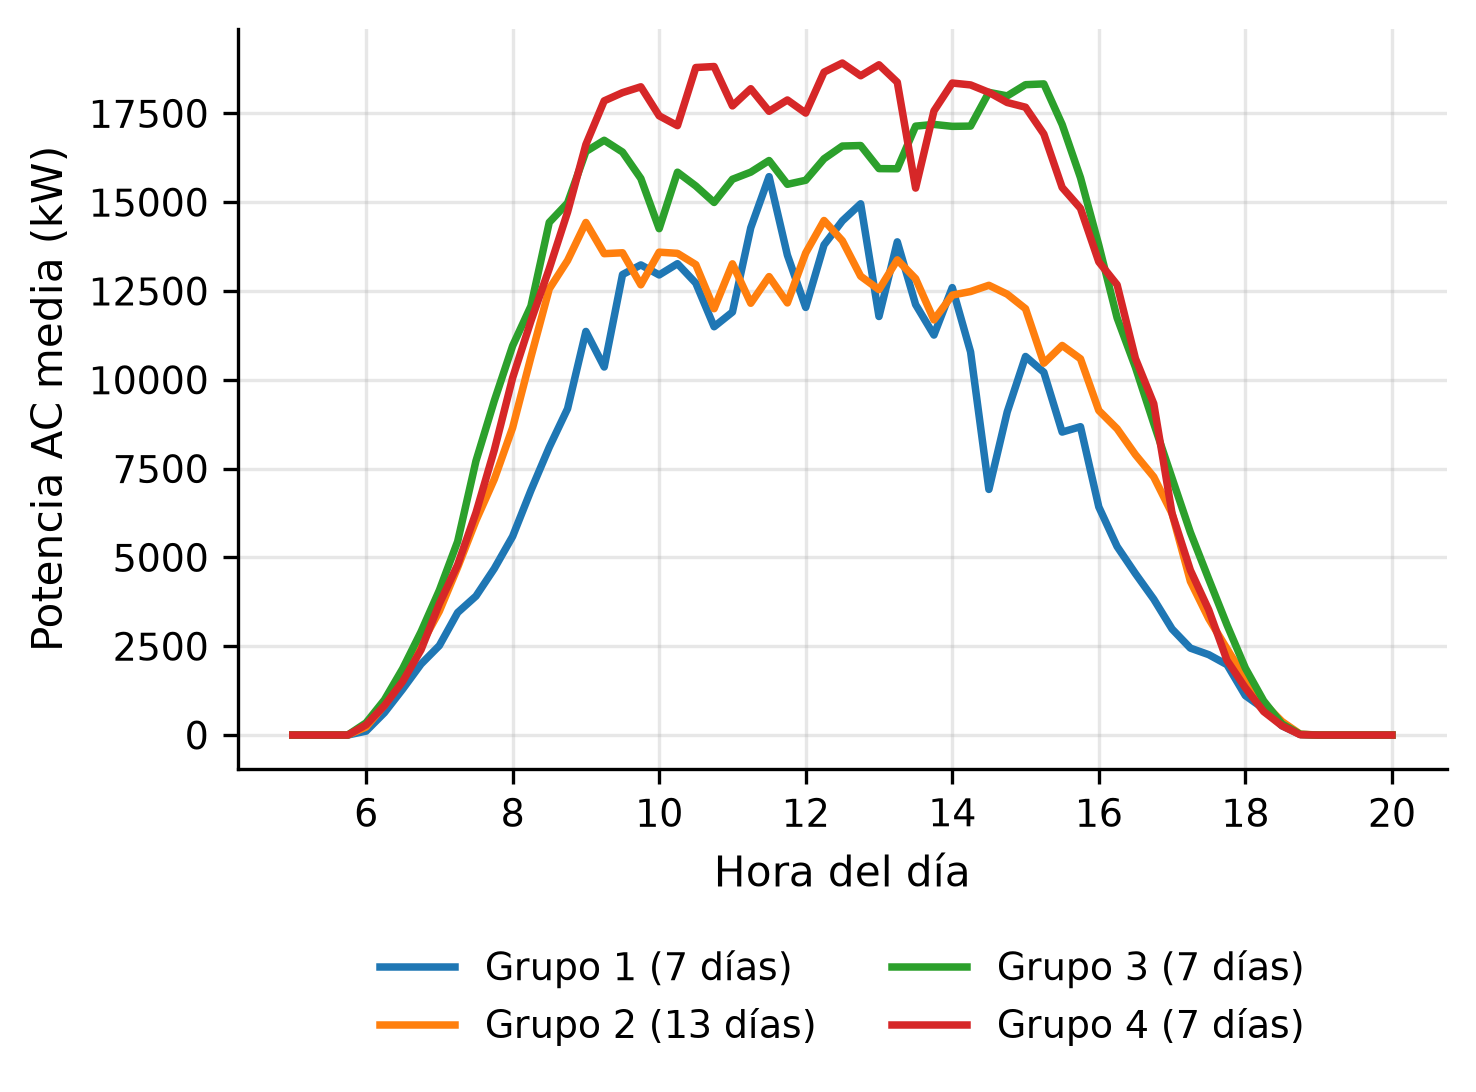
\includegraphics[width=\columnwidth]{fig_grupos.png}
\caption{Perfil medio de potencia de cada grupo de d\'ias: 1, nublado con pocas p\'erdidas; 2, parcialmente nublado con p\'erdidas; 3, despejado con p\'erdidas moderadas; 4, despejado con pocas p\'erdidas.}
\label{fig:grupos}
\end{figure}

\section{Discusi\'on}
Los resultados dejan una imagen coherente: ganarle a la persistencia es dif\'icil, el clima reciente casi no a\~nade informaci\'on y los errores se concentran donde la planta pierde inversores. Cada una de esas piezas responde una de las preguntas planteadas.

\subsection{P1: cu\'anto mejora el ensamble a la persistencia}
En la semana de prueba, el ensamble subi\'o el F1 macro de \tPersFmacro{} a \tEnsFmacro{} y $\kappa$ de \tPersKappa{} a \tEnsKappa{} (Tabla~\ref{tab:resultados}); en los 14 d\'ias de confirmaci\'on, la ventaja fue de \wfPersFmacro{} en F1 macro y \wfPersKappa{} en $\kappa$, con intervalos que excluyen el cero. La mejora es real pero modesta, y la raz\'on est\'a en la propia serie: a 15~min el nivel casi no cambia, as\'i que repetir el \'ultimo ya acierta la mayor\'ia de las veces y el margen que queda est\'a en las transiciones. Ah\'i ning\'un modelo suelto se despeg\'o, y por eso la ganancia vino de combinar modelos que se equivocan en momentos distintos \cite{dietterich}. La Fig.~\ref{fig:combinatoria} explica, a la vez, por qu\'e no se eligi\'o el primer puesto: con una correlaci\'on de \spearman{} entre desarrollo y confirmaci\'on, el ranking de 6 d\'ias es en buena parte azar, y solo una combinaci\'on que se mantiene arriba en todas las evaluaciones merece confianza. Aun as\'i, esa elecci\'on us\'o los mismos d\'ias que se reportan; corregida con selecci\'on anidada, la ventaja sobre la combinaci\'on persistencia-climatolog\'ia baja a \anidFmacro{} en F1 macro y \anidKappa{} en $\kappa$ \cite{cawley}. Frente a esa combinaci\'on, adem\'as, el ensamble no mejora la precisi\'on de bajo (\wfCombPrec{} [\wfCombPrecLo{}; \wfCombPrecHi{}]).

Para la empresa, lo que importa de esa mejora es cu\'anto se equivoca al anunciar bajo. El ensamble cometi\'o \tEnsFalsosBajo{} falsos bajo frente a \tPersFalsosBajo{} de la persistencia, y la energ\'ia en juego baj\'o de \tPersMWh{} a \tEnsMWh{}~MWh. Hay que ser honestos con el ahorro, sin embargo: elegir las horas con el ensamble ahorra el \ahorroEns{}~\% del costo de intervenir sin criterio, pero una regla de horario sin modelo, que solo evita el mediod\'ia, ya ahorra el \ahorroRegla{}~\%. El valor del modelo no est\'a en los pesos que ahorra sobre una regla simple, sino en intervenir menos veces con la planta produciendo y en aprovechar las ventanas bajas reales (recall de \tEnsRec{}).

\subsection{P2: cu\'anto aporta el clima reciente}
Si la ventaja es tan estrecha, cabe preguntar si el sensor ayuda a ampliarla. La respuesta es que no: con solo la historia de la potencia (A) el F1 macro fue \fConjA{}, con ambos (C) \fConjC{} y con solo el clima (B) \fConjB{}; en kilovatios, la habilidad frente a la persistencia fue \habA{} con A y \habB{} con B. La causa es que la potencia de hace 15~min ya contiene el efecto de la irradiancia (su correlaci\'on con la potencia siguiente es de \corrpot{}, frente a \corrirr{} de la irradiancia), y adem\'as incorpora lo que el sensor no ve: el recorte del inversor \cite{good}, la temperatura del m\'odulo \cite{skoplaki} y los inversores ca\'idos. Las reglas del \'arbol lo muestran de forma muy legible. El nivel bajo queda casi resuelto cuando $G_{t-1}\le\reglaBajoGuno{}$ y $G_{t-4}\le\reglaBajoGcuatro{}$~kW/m$^2$ (el \reglaBajoPct{}~\% del entrenamiento, con pureza de \reglaBajoPureza{}~\%), y el alto, cuando $G_{t-1}>\reglaAltoG{}$~kW/m$^2$ y $P_{t-1}>\reglaAltoP{}$~kW (\reglaAltoPct{}~\%, pureza de \reglaAltoPureza{}~\%). El \'arbol corta por irradiancia, pero lo hace porque irradiancia y potencia reciente cargan la misma informaci\'on. Entre ambas reglas queda el nivel medio, con hojas de pureza cercana al 70~\%, y es justo ah\'i donde la matriz de confusi\'on concentra el error.

Que estos resultados sean modestos es, de hecho, una buena se\~nal. Al agregar la potencia DC del mismo instante, el \'arbol pasa de una exactitud de \fugaAccSin{} a \fugaAccCon{} y de un $\kappa$ de \fugaKappaSin{} a \fugaKappaCon{}: un resultado casi perfecto que ser\'ia un espejismo, porque esa variable no existe cuando se pronostica. El sensor no sirve para mejorar el pron\'ostico, pero s\'i para lo que el pron\'ostico no puede hacer: comparar lo que la planta deber\'ia producir con lo que produce.

\subsection{P3: d\'onde falla y por qu\'e}
Esa comparaci\'on es la que explica los errores. En los d\'ias parcialmente nublados con p\'erdidas, el error fue de \gDosErr{}~\% frente a \gUnoErr{}~\% en los nublados con pocas p\'erdidas, y la diferencia no est\'a en las nubes sino en los inversores en cero (\gDosInv{} frente a \gUnoInv{} en promedio). Cuando el ensamble anunci\'o un nivel m\'as alto que el real hab\'ia \invsobre{} inversores en cero, y en los \iecConN{} instantes con inversores en cero su F1 macro cae de \iecSinEnsFmacro{} a \iecConEnsFmacro{}. La causa es operativa: un inversor que se desconecta hunde la potencia sin que nada en el pasado inmediato lo anuncie, y en esos d\'ias ning\'un modelo basado en historia puede anticiparlo. Aun en ese subconjunto, el ensamble cometi\'o \iecConEnsFalsosBajo{} falsos bajo frente a \iecConPersFalsosBajo{} de la persistencia. La implicaci\'on es que el error del modelo es en s\'i mismo una se\~nal: si anuncia alto o medio y la planta genera bajo, el t\'ecnico debe revisar el MPPT del inversor, la suciedad \cite{diazgranados,costa}, las sombras parciales \cite{yaouba,maki} o los strings desconectados.

\subsection{Limitaciones, \'etica e impactos}
Estas respuestas tienen un alcance acotado. Es una sola planta y un solo mes de la India; la semana de prueba fue m\'as nublada que el entrenamiento, solo tuvo \naltotest{} instantes altos y solo dos de los cuatro tipos de d\'ia, as\'i que nada puede decirse de los d\'ias despejados. Las cifras miden el m\'etodo, no el desempe\~no en una planta colombiana, y el costo en pesos depende de un precio supuesto. La Tabla~\ref{tab:etica} re\'une estos l\'imites junto con los dilemas \'eticos y los impactos del uso del modelo, cada uno con su mitigaci\'on.

\begin{table}[t]
\caption{Dilemas \'eticos e impactos, con su mitigaci\'on}
\label{tab:etica}
\centering
\footnotesize
\setlength{\tabcolsep}{3pt}
\begin{tabular}{@{}p{0.2\columnwidth}p{0.36\columnwidth}p{0.38\columnwidth}@{}}
\toprule
Aspecto & Riesgo & Mitigaci\'on \\
\midrule
Privacidad & Ninguno: los datos son de equipos, no de personas & Ninguna columna identifica a una persona \\
Uso responsable & Un falso bajo hace intervenir con producci\'on; un falso alto oculta fallas & Reportar la energ\'ia de los falsos bajo; umbral opcional para bajo \\
Transparencia & Sobrevender una mejora peque\~na & Reportar los \ncandidatos{} modelos, las \ncombinaciones{} combinaciones y la ganancia corregida \\
Sesgo de datos & Una planta, un mes, otro pa\'is & Reentrenar y recalcular los terciles con datos colombianos \\
Seguridad & Mandar a intervenir equipos energizados & La alerta recomienda; se siguen los protocolos de la empresa \\
\midrule
Social & Confiar de m\'as y descuidar la inspecci\'on & El t\'ecnico decide; la alerta trae hora y causa probable \\
Econ\'omico & Sobrestimar el ahorro con un precio supuesto & Reportar tambi\'en MWh; usar el precio real del contrato \\
Ambiental & Huella del c\'omputo en la nube & Modelo liviano; reentrenar cada mes, no a diario \\
Global & Extrapolar cifras de un clima a otro & Reentrenar por planta; m\'etodo replicable con SCADA est\'andar \\
\bottomrule
\end{tabular}
\end{table}

\section{Conclusiones y despliegue}
Las tres respuestas convergen en una conclusi\'on: con estos datos, anticipar el nivel de la planta 15~min antes es posible y \'util, pero la mejora sobre la persistencia es peque\~na, y el valor del modelo est\'a en lo que la persistencia no hace. El ensamble de cuatro modelos le gana en F1 macro y $\kappa$ con intervalos que excluyen el cero, comete menos falsos bajo y, sobre todo, convierte su propio error en una se\~nal de falla. La historia de la potencia contiene casi todo lo que se puede saber a ese horizonte, y la combinaci\'on exhaustiva de modelos solo mereci\'o confianza cuando se eligi\'o por consistencia y se corrigi\'o el sesgo de selecci\'on.

En la operaci\'on, el modelo lo usar\'ia el centro de control de la empresa cada 15~min, con el registro nuevo de la planta y los mismos rezagos y limpieza de este trabajo; en una simulaci\'on fila a fila, la funci\'on de pron\'ostico reprodujo el \psimcoincide{}~\% de las predicciones por lotes. Cuando anuncia bajo, el t\'ecnico puede programar la intervenci\'on; cuando anunci\'o alto o medio y la planta genera bajo, o hay inversores en cero con sol, se emite una alerta con la lista de causas probables, que el t\'ecnico confirma en campo. El modelo se reentrena cada mes con los terciles recalculados por planta, y se retira, volviendo a la persistencia, si su precisi\'on de bajo cae por debajo de la de esta durante dos semanas. El riesgo principal es la estaci\'on: un clima ausente del entrenamiento cambia el significado de bajo, medio y alto.

Para que esta base se convierta en una herramienta para Colombia hacen falta tres mejoras: m\'as meses y plantas colombianas para repetir la comparaci\'on con los mismos pasos, pron\'osticos de irradiancia que anuncien las nubes que la historia no ve, y registros de mantenimiento que permitan confirmar las causas que hoy la alerta solo propone. Separar desde el inicio los d\'ias de selecci\'on y de reporte evitar\'ia, adem\'as, el sesgo que aqu\'i solo pudo medirse despu\'es.

\section*{Declaraci\'on de uso de IAG}
Este trabajo se desarroll\'o en el Nivel~3 de colaboraci\'on con IAG. Se us\'o Claude (Anthropic) para depurar c\'odigo, sugerir el c\'odigo de las figuras, organizar el cuaderno y apoyar la redacci\'on de este informe. Todo el c\'odigo se ejecut\'o y revis\'o en el cuaderno, las cifras del informe se generan autom\'aticamente desde sus salidas y las fuentes se verificaron en el documento original o en su resumen. Las decisiones de preparaci\'on de los datos, la elecci\'on de los modelos, la interpretaci\'on y la discusi\'on son del grupo.

\begin{thebibliography}{99}
\footnotesize
\bibitem{ley1715} Congreso de la Rep\'ublica de Colombia, ``Ley 1715 de 2014: por medio de la cual se regula la integraci\'on de las energ\'ias renovables no convencionales al Sistema Energ\'etico Nacional,'' \emph{Diario Oficial} n.\textordmasculine~49150, Bogot\'a, Colombia, may. 2014.
\bibitem{ley2099} Congreso de la Rep\'ublica de Colombia, ``Ley 2099 de 2021: por medio de la cual se dictan disposiciones para la transici\'on energ\'etica, la dinamizaci\'on del mercado energ\'etico, la reactivaci\'on econ\'omica del pa\'is y se dictan otras disposiciones,'' \emph{Diario Oficial} n.\textordmasculine~51.731, Bogot\'a, Colombia, jul. 2021.
\bibitem{xm} XM S.A. E.S.P., ``Capacidad solar en operaci\'on y en pruebas,'' Sistema de Informaci\'on del Mercado de Energ\'ia Mayorista (SIMEM), serie anual 2021--2026. [En l\'inea]. Disponible: \url{https://www.simem.co}
\bibitem{skoplaki} E. Skoplaki y J. A. Palyvos, ``On the temperature dependence of photovoltaic module electrical performance: A review of efficiency/power correlations,'' \emph{Solar Energy}, vol.~83, n.\textordmasculine~5, pp.~614--624, 2009.
\bibitem{good} J. Good y J. X. Johnson, ``Impact of inverter loading ratio on solar photovoltaic system performance,'' \emph{Applied Energy}, vol.~177, pp.~475--486, 2016, doi: 10.1016/j.apenergy.2016.05.134.
\bibitem{diazgranados} J. D. Diazgranados-Garz\'on \emph{et al.}, ``Analysis of the soiling effect on solar-panel power efficiency in the Colombian Caribbean region,'' \emph{Revista Facultad de Ingenier\'ia Universidad de Antioquia}, n.\textordmasculine~97, pp.~22--29, 2020.
\bibitem{costa} S. C. S. Costa, L. L. Kazmerski y A. S. A. C. Diniz, ``Impact of soiling on Si and CdTe PV modules: Case study in different Brazil climate zones,'' \emph{Energy Conversion and Management: X}, vol.~10, art.~100084, 2021, doi: 10.1016/j.ecmx.2021.100084.
\bibitem{yaouba} Yaouba \emph{et al.}, ``An experimental and case study on the evaluation of the partial shading impact on PV module performance operating under the Sudano-Sahelian climate of Cameroon,'' \emph{Frontiers in Energy Research}, vol.~10, art.~924285, 2022, doi: 10.3389/fenrg.2022.924285.
\bibitem{maki} A. M\"aki y S. Valkealahti, ``Power losses in long string and parallel-connected short strings of series-connected silicon-based photovoltaic modules due to partial shading conditions,'' \emph{IEEE Trans. Energy Convers.}, vol.~27, n.\textordmasculine~1, pp.~173--183, 2012.
\bibitem{cantillo} S. Cantillo-Luna, R. Moreno-Chuquen, D. Celeita y G. Anders, ``Deep and machine learning models to forecast photovoltaic power generation,'' \emph{Energies}, vol.~16, n.\textordmasculine~10, art.~4097, 2023, doi: 10.3390/en16104097.
\bibitem{theocharides} S. Theocharides, G. Makrides y G. E. Georghiou, ``PV generation forecasting utilizing a classification-only approach,'' \emph{EPJ Photovoltaics}, vol.~15, art.~12, 2024, doi: 10.1051/epjpv/2024011.
\bibitem{santiago} I. Santiago, J. L. Esquivel-Martin, D. Trillo-Montero, R. J. Real-Calvo y V. Pall\'ares-L\'opez, ``Classification of daily irradiance profiles and the behaviour of photovoltaic plant elements: The effects of cloud enhancement,'' \emph{Applied Sciences}, vol.~11, n.\textordmasculine~11, art.~5230, 2021, doi: 10.3390/app11115230.
\bibitem{clemen} R. T. Clemen, ``Combining forecasts: A review and annotated bibliography,'' \emph{Int. J. Forecasting}, vol.~5, n.\textordmasculine~4, pp.~559--583, 1989, doi: 10.1016/0169-2070(89)90012-5.
\bibitem{kaggle} A. Kannal, ``Solar power generation data,'' Kaggle, 2020. [En l\'inea]. Disponible: \url{https://www.kaggle.com/datasets/anikannal/solar-power-generation-data}
\bibitem{crispdm} IBM Corporation, \emph{Gu\'ia de CRISP-DM de IBM SPSS Modeler}, versi\'on 18.4. Armonk, NY, EE.~UU.: IBM.
\bibitem{iec61724} \emph{Photovoltaic System Performance -- Part 1: Monitoring}, IEC 61724-1:2021, ed.~2.0, International Electrotechnical Commission, Ginebra, Suiza, 2021.
\bibitem{dietterich} T. G. Dietterich, ``An experimental comparison of three methods for constructing ensembles of decision trees: Bagging, boosting, and randomization,'' \emph{Machine Learning}, vol.~40, n.\textordmasculine~2, pp.~139--157, 2000.
\bibitem{wang} X. Wang, R. J. Hyndman, F. Li y Y. Kang, ``Forecast combinations: An over 50-year review,'' arXiv:2205.04216, 2022, doi: 10.48550/arXiv.2205.04216.
\bibitem{smith} J. Smith y K. F. Wallis, ``A simple explanation of the forecast combination puzzle,'' \emph{Oxford Bull. Econ. Statist.}, vol.~71, n.\textordmasculine~3, 2009, doi: 10.1111/j.1468-0084.2008.00541.x.
\bibitem{cawley} G. C. Cawley y N. L. C. Talbot, ``On over-fitting in model selection and subsequent selection bias in performance evaluation,'' \emph{J. Mach. Learn. Res.}, vol.~11, n.\textordmasculine~70, pp.~2079--2107, 2010.
\bibitem{reforms} S. Kapoor \emph{et al.}, ``REFORMS: Consensus-based recommendations for machine-learning-based science,'' \emph{Science Advances}, 2024, doi: 10.1126/sciadv.adk3452.
\bibitem{python} Python Software Foundation, \emph{The Python Language Reference}, versi\'on 3.13. [En l\'inea]. Disponible: \url{https://docs.python.org/3/reference/}
\bibitem{numpy} C. R. Harris \emph{et al.}, ``Array programming with NumPy,'' \emph{Nature}, vol.~585, n.\textordmasculine~7825, pp.~357--362, 2020, doi: 10.1038/s41586-020-2649-2.
\bibitem{pandas} W. McKinney, ``Data structures for statistical computing in Python,'' en \emph{Proc. 9th Python in Science Conf.}, 2010, pp.~56--61, doi: 10.25080/Majora-92bf1922-00a.
\bibitem{sklearn} F. Pedregosa \emph{et al.}, ``Scikit-learn: Machine learning in Python,'' \emph{J. Mach. Learn. Res.}, vol.~12, pp.~2825--2830, 2011.
\bibitem{xgboost} T. Chen y C. Guestrin, ``XGBoost: A scalable tree boosting system,'' en \emph{Proc. 22nd ACM SIGKDD Conf. Knowledge Discovery and Data Mining}, 2016, arXiv:1603.02754.
\bibitem{scipy} P. Virtanen \emph{et al.}, ``SciPy 1.0: Fundamental algorithms for scientific computing in Python,'' \emph{Nature Methods}, vol.~17, n.\textordmasculine~3, pp.~261--272, 2020, doi: 10.1038/s41592-019-0686-2.
\bibitem{statsmodels} S. Seabold y J. Perktold, ``statsmodels: Econometric and statistical modeling with Python,'' en \emph{Proc. 9th Python in Science Conf.}, 2010.
\bibitem{matplotlib} J. D. Hunter, ``Matplotlib: A 2D graphics environment,'' \emph{Comput. Sci. Eng.}, vol.~9, n.\textordmasculine~3, pp.~90--95, 2007, doi: 10.1109/MCSE.2007.55.
\bibitem{seaborn} M. L. Waskom, ``seaborn: Statistical data visualization,'' \emph{J. Open Source Softw.}, vol.~6, n.\textordmasculine~60, art.~3021, 2021, doi: 10.21105/joss.03021.
\bibitem{missingno} A. Bilogur, ``Missingno: A missing data visualization suite,'' \emph{J. Open Source Softw.}, vol.~3, n.\textordmasculine~22, art.~547, 2018, doi: 10.21105/joss.00547.
\bibitem{joblib} Joblib developers, \emph{Joblib: Running Python functions as pipeline jobs}, versi\'on 1.6.0. [En l\'inea]. Disponible: \url{https://joblib.readthedocs.io}
\bibitem{ipython} IPython developers, \emph{IPython: Productive interactive computing}. [En l\'inea]. Disponible: \url{https://ipython.org}
\end{thebibliography}

\end{document}
